

\documentclass[norsk,twoside,utf8]{article}
\usepackage{lipsum} % Package to generate dummy text throughout this template
\usepackage{comment}
\usepackage{amsmath, amssymb}
\usepackage{eulervm}

\usepackage{graphicx}
\usepackage{tikz}
\usetikzlibrary{calc,intersections,patterns}
\usepackage{epigraph}
\usepackage[lined,boxed,commentsnumbered]{algorithm2e}
\usepackage[utf8]{inputenc}
\usepackage{listings}
\usepackage[T1]{fontenc} % Use 8-bit encoding that has 256 glyphs
\usepackage{microtype} % Slightly tweak font spacing for aesthetics
\usepackage[hmarginratio=1:1,top=32mm,columnsep=20pt]{geometry} % Document margins
\usepackage{multicol} % Used for the two-column layout of the document
\usepackage[hang, small,labelfont=bf,up,textfont=it,up]{caption} % Custom captions under/above floats in tables or figures
\usepackage{booktabs} % Horizontal rules in tables
\usepackage{float} % Required for tables and figures in the multi-column environment - they need to be placed in specific locations with the [H] (e.g. \begin{table}[H])
\usepackage[hyperfootnotes=false]{hyperref} % For hyperlinks in the PDF
\usepackage{lettrine} % The lettrine is the first enlarged letter at the beginning of the text
\usepackage{paralist} % Used for the compactitem environment which makes bullet points with less space between them
\usepackage{abstract} % Allows abstract customization
\usepackage{titlesec} % Allows customization of titles

\renewcommand{\abstractname}{Sammendrag}
\renewcommand\refname{Kilder}
\renewcommand{\abstractnamefont}{\normalfont\bfseries} % Set the "Abstract" text to bold
\renewcommand{\abstracttextfont}{\normalfont\small\itshape} % Set the abstract itself to small italic text
\renewcommand\thesection{\Roman{section}} % Roman numerals for the sections
\renewcommand\thesubsection{\roman{subsection}} % Roman numerals for subsections
\titleformat{\section}[block]{\large\scshape\centering\bfseries}{\thesection.}{1em}{} % Change the look of the section titles
\titleformat{\subsection}[block]{\scshape\bfseries}{\thesubsection.}{1em}{} % Change the look of the section titles
%\renewcommand{ \figurename }{ Figur }


\newcommand{\EQU}[1] { \begin{equation*} \begin{split} #1 \end{split} \end{equation*} }
\newcommand{\EQUn}[1] { \begin{equation} \begin{split} #1 \end{split} \end{equation} }
\newcommand{\PAR}[2]{ \frac{\partial #1}{\partial #2}}
\newcommand{\ket}[1] { |#1\rangle }
\newcommand{\expe}[1]{ \langle #1 \rangle }
\newcommand{\bra}[1] { \langle #1 | }
\newcommand{\braket}[2] { \langle #1 | #2 \rangle }


%%%%********************************************************************
\usepackage{microtype} 
\usepackage{graphicx}
\usepackage{xcolor}
\usepackage{lipsum}

%%%%********************************************************************
% fancy quotes
\definecolor{quotemark}{gray}{0.7}
\makeatletter
\def\fquote{%
    \@ifnextchar[{\fquote@i}{\fquote@i[]}%]
           }%
\def\fquote@i[#1]{%
    \def\tempa{#1}%
    \@ifnextchar[{\fquote@ii}{\fquote@ii[]}%]
                 }%
\def\fquote@ii[#1]{%
    \def\tempb{#1}%
    \@ifnextchar[{\fquote@iii}{\fquote@iii[]}%]
                      }%
\def\fquote@iii[#1]{%
    \def\tempc{#1}%
    \vspace{1em}%
    \noindent%
    \begin{list}{}{%
         \setlength{\leftmargin}{0.1\textwidth}%
         \setlength{\rightmargin}{0.1\textwidth}%
                  }%
         \item[]%
         \begin{picture}(0,0)%
         \put(-15,-5){\makebox(0,0){\scalebox{4}{\textcolor{quotemark}{''}}}}%
         \end{picture}%
         \begingroup\itshape}%
 %%%%********************************************************************
 \def\endfquote{%
 \endgroup\par%
 \makebox[0pt][l]{%
 \hspace{0.8\textwidth}%
 \begin{picture}(0,0)(0,0)%
 \put(15,15){\makebox(0,0){%
 \scalebox{4}{\color{quotemark}''}}}%
 \end{picture}}%
 \ifx\tempa\empty%
 \else%
    \ifx\tempc\empty%
       \hfill \mbox{}\hfill\tempa\ \emph{\tempb}%
   \else%
       \hfill \mbox{}\hfill\tempa,\ \emph{\tempb},\ \tempc%
   \fi\fi\par%
   \vspace{0.5em}%
 \end{list}%
 }%

%----------------------------------------------------------------------------------------
%	TITLE SECTION
%----------------------------------------------------------------------------------------

\title{\vspace{-15mm}\fontsize{24pt}{10pt}\selectfont\textbf{MAT2500 \\ Prosjektoppgave \\ En hyllest til Euklid}} % Article title
\author{
\large
\textsc{
August Geelmuyden
} \\
\normalsize Universitetet i Oslo \\ % Your institution
\vspace{-5mm}
}
\date{}

%----------------------------------------------------------------------------------------

\begin{document}

\maketitle % Insert title

%----------------------------------------------------------------------------------------
%	ABSTRACT
%----------------------------------------------------------------------------------------

\begin{abstract}

\noindent
I tredje bind av Euklids trettenbindsverk Elementer studeres proposisjon 35. Først undersøkes måten matematiske påstander ble formulert før den matematiske formalisme oppstod, deretter omtales resultatene som utgjør fundamentet for proposisjon 35 bind i tredje bind. Deretter er forsøk gjort på å modernisere beviset av proposisjonen. Videre følger en diskusjon av det matematiske innholdet i utsagnet. Proposisjonen kan sies å være forgjengeren til teorien rundt punktets potens, som er et spesialtilfelle av Darbouxproduktet mellom to sirkler. For to sirkler oppdages det at mengden av punkter med lik potens med hensyn på begge sirklene er en rett linje -- potenslinjen. 

\end{abstract}

%----------------------------------------------------------------------------------------
%	ARTICLE CONTENTS
%----------------------------------------------------------------------------------------


\section{Euklids elementer}
 \begin{fquote}[E. T. Bell]
  Euclid taught me that without assumptions there is no proof. Therefore, in any argument, examine the assumptions.
 \end{fquote}

\noindent
Det er vanskelig ikke å la seg fascinere av Euklids trettenbindsverk \textit{Elementer}. Bøkene, som ble skrevet av den greske matematikeren Euklid rundt 300 år før vår tidsregning, fungerte som standard lærebok i geometri helt frem til det 20. århundre. Elementer ble altså ikke bare skrevet lenge før standard regnesymboler som $+,-,\times,/,\sqrt{}$ og $=$ ble introdusert -- verket ble skrevet hele 1600 år før Europa byttet fra romertall til det hindu-arabiske tallsystemet vi har i dag. Hva er det med Euklids elementer som gjør at ingen fikk til å forbedre læreverket på hele 2200 år? 






\section{Oppbygning}
\subsection{Et sammensatt verk}

Noe av det som er særegent med Euklids elementer er verkets oppbygning. Han begynner første bind med 23 definisjoner. Først konstateres det at et \textit{punkt} er det som ikke kan deles og at en \textit{linje} er en lengde uten bredde. I den femtende definisjonen fremlegger han videre hva som skal menes med ordet \textit{sirkel} -- nemlig den plane figuren som har et indre punkt med den egenskapen at alle rette linjer fra punktet som faller på figurens rand er like. Punktet kaller han for sirkelens \textit{sentrum}. 

Etter definisjonene kommer hans fem posutlater. Disse er så viktige at de fortjener en plass i denne teksten:
\begin{itemize}
\item[1.] Mellom to punkter kan alltid en rett linje tegnes.
\item[2.] Fra en rett linje kan det kontinuerlig produseres endelige rette linjer. 
\item[3.] En sirkel kan alltid trekkes, uavhengig av sentrum og radius. 
\item[4.] Alle rette vinkler er like.
\item[5.] To linjer som ikke er parallelle vil møtes på den siden der de indre vinklene er mindre en to rette vinkler.
\end{itemize}
Før Euklid er klar for å bygge opp matematikken fra bunnen av lister han opp fem alminnelige observasjoner. Her konstaterer han for eksempel at ting som er lik det samme, er også lik hverandre og at det hele alltid er større en dets bestanddeler. 

Euklid begynner så sin konstruksjon av matematikken. Hver proposisjon bygger på tidligere utsagn, som til slutt bunner ut i definisjoner, postulater og alminnelige observasjoner. Hvert bind bygger på de foregående. I første bind dreier stort sett alt seg om trekanter. Det er da naturlig at andre bind omhandler rektangler. Før polygoner angripes i fjerde bind introduserer Euklid teorien rundt sirkler i tredje bind. Deretter tar han for seg proporsjonalitet og similaritet før han vier syvende, åttende, niende og tiende bind til tallteori. De tre siste bindene omhandler geometri i rommet, pyramider og til slutt platonske legemer. En nevneverdig forskjell fra vår tids matematikk er innholdet i proposisjonene. Proposisjonene kan deles inn i to grupper. Den ene er proposisjoner med argumenter som avsluttes med \textit{Q.E.D.}(\textit{quod erat demonstrandum}), som betyr \textit{det som skulle vises}. Disse er de moderne proposisjonene. Den andre typen har argumenter som ender med \textit{Q.E.F}(\textit{quod erat faciendum}), som betyr \textit{det som skulle gjøres}. Proposisjoner av denne typen dreier seg om den tekniske utførelsen av et geometrisk argument. Blant proposisjonene finner du altså også setninger som ''hvordan tegne en rett linje vinkelrett på en annen'' og ''hvordan dele et rett linjestykke i to like store deler''.



\subsection{Fundamentet for proposisjon 35 i tredje bind}
Denne prosjektoppgaven skal i hovedsak beskjeftige seg med den 35. proposisjonen i verkets tredje bind. Å ramse opp Euklids påstand og argument vil imidlertid ha lite for seg uten først å nevne hvilke utsagn proposisjonen hviler på. 

Proposisjon 35, bind 3, hviler i hovedsak bare på fem tidligere utsagn. Disse er som følger:
\begin{multicols}{2}

\begin{figure}[H]
\begin{center}
\includegraphics*[width=0.5\textwidth]{oppbygg.png}
\end{center}
\caption{
Grafen viser hvilke utsagn proposisjon 35 i tredje bind baserer seg på, og hvilke utsagn utsagnene baserer seg på. 
}
\label{oppbygg}
\end{figure}

\begin{description}
\item[III.1] Hvordan finne sentrum i en gitt sirkel.
\item[I.12] Hvordan trekke en rett linje vinkelrett på en gitt rett linje fra et punkt som ikke ligger på den.
\item[III.3] Hvis en rett linje fra sentrum i en sirkel deler en rett linje, som ikke går gjennom sentrum, i to like deler, da står linjene normalt på hverandre. Hvis linjene står normalt på hverandre deles linjen som ikke går gjennom sentrum i to like deler. 
\item[II.5] Hvis en rett linje deles i like og ulike segmenter, da er rektangelet av de ulike segmentene til hele linjen sammen med kvadratet på den rette linjen mellom skjæringspunktene lik kvadratet på halve linjen. 
\item[I.47] I en rettvinklet trekant er kvadratet på motsatt side av den rette vinkelen lik summen av kvadratene på sidene som inneholder den rette vinkelen.
\end{description}

\end{multicols}

\noindent
Legg merke til hvordan de to første proposisjonene dreier seg om den tekniske utførelsen av konstruksjonen. I moderne argumentasjon vil man ikke behøve å referere til en metode for å finne sentrum i en sirkel. I dag er det mer nødvendig å bemerke eksistens og utvetydighet av et sentrum enn det er å kunne metoden for å finne et eventuelt sentrum. Blant de fem proposisjonene finner du kanskje også en gammel kjenning. Proposisjon $I.47$ er nemlig det vi kjenner som \textit{Pythagoras læresetning}. Setningen antas velkjent, men ordbruken er verdt å bemerke. I $I.47$ bruker verken algebra eller ord som hypotenus og katet for å fastslå den velkjente likheten; alt som brukes er kvadrater og deres posisjon relativt til den rette vinkelen. 

\begin{multicols}{2}
\begin{center}
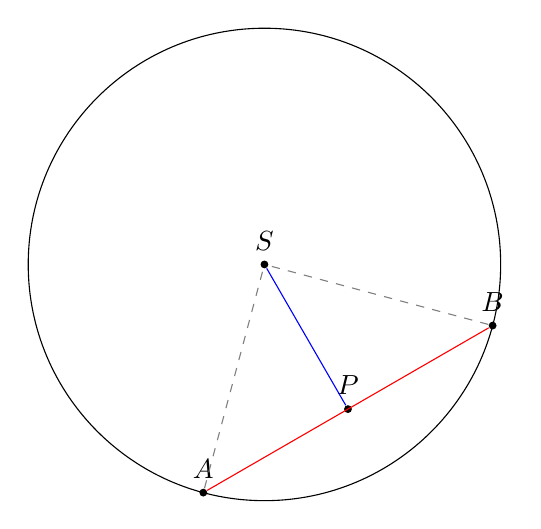
\begin{tikzpicture}[
  dot/.style={circle,inner sep=1pt,fill,label={#1},name=#1},
  dot2/.style={circle,inner sep=1pt,fill},
  extended line/.style={shorten >=-#1,shorten <=-#1},
  extended line/.default=1cm
  ]
\def\radius{3}
\def\ptRadius{0.05} 
\def\at{180+75}
\def\bt{270+75} 
\node[dot=$A$] (A) at ({\radius*cos(\at)},{\radius*sin(\at)}){};   % point on circle
\node[dot=$B$] (B) at ({\radius*cos(\bt)},{\radius*sin(\bt)}){};   % point on circle
\node[dot=$S$] (S) at (0,0){};                                     % center
\node[dot=$P$] (P) at ($(A)!(S)!(B)$){};           				 % normal from S
\draw (S) circle (\radius);
\draw[red]  (A) -- (B);
\draw[blue] (S) -- (P);
\draw[gray,dashed] (A) -- (S);
\draw[gray,dashed] (B) -- (S);
\end{tikzpicture}
\end{center}
\vspace{1cm}
\noindent
Proposisjon $III.3$, som er en ganske eksakt replika av et korrolar til konstruksjonen i $III.1$, er en påminnelse om et intuitivt faktum om rette linjer i sirkler. Hvis $A$ og $B$ er to punkter på en sirkel med sentrum $S$, da deler linjen $SP$ som står normalt på $AB$ linjen $AB$ i to like store deler. For å innse dette kan vi bruke pythagoras til å fastslå at $AP^2 = PS^2 + SA^2$ og siden $SA=SB$ er radien i sirkelen må $AP^2=PS^2+SB^2 = BP^2$. 

I $III.3$ nevnes også det motsatte; hvis $AB$ deles i to like store deler av et punkt $P$, må $PS$ stå normalt på $AB$. At dette er sant kan erkjennes ved å konstatere at $AS=BS$ er radien, $AP=PB$ er antakelsen og $EF$ er en delt side for trekantene $\Delta ASP$ og $\Delta BSP$. Derfor må vinkelene $\angle APS$ og $\angle BPS$ være like, og siden $\angle APB$ er $180^\circ$ må $SP$ stå normalt på $AB$.
\end{multicols}
Den mest kryptiske av proposisjonene brukt i $III.35$ er trolig $II.5$. Denne må vi se litt nærmere på for å uskadeliggjøre. 

\subsection{Proposisjon 5 bind 2}
Utsagnet sier at hvis en rett linje $AB$ deles på midten av et punkt $C$ og i ulike deler av et punkt $D$, så er 
rektangelet $AD$ ved $DB$ sammen med kvadratet $CD$ lik kvadratet $CB$. 
\begin{multicols}{2}
\begin{center}
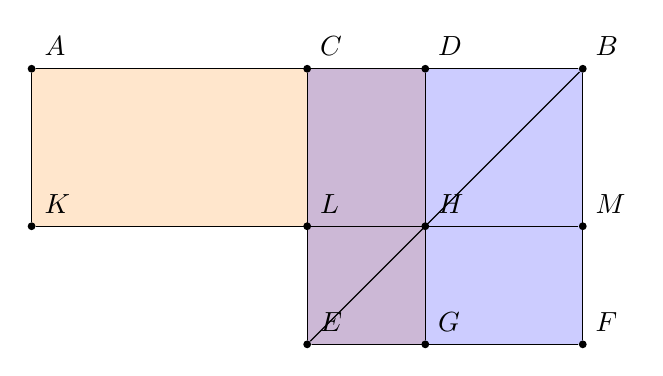
\begin{tikzpicture}[
  dot/.style={circle,inner sep=1pt,fill,label=above right:{#1},name=#1},
  dot2/.style={circle,inner sep=1pt},
  extended line/.style={shorten >=-#1,shorten <=-#1},
  extended line/.default=1cm
  ]
\def\aa{0}
\def\bb{7} 
\def\cc{0.5*\bb-0.5*\aa}
\def\dd{5} 
\node[dot2=A] (A) at (\aa,0){};   
\node[dot2=B] (B) at (\bb,0){};  
\node[dot2=C] (C) at (\cc,0){};      
\node[dot2=D] (D) at (\dd,0){};  
\node[dot2=M] (M) at (\bb,\dd-\bb){};  
\node[dot2=H] (H) at (\dd,\dd-\bb){};  
\node[dot2=L] (L) at (\cc,\dd-\bb){};  
\node[dot2=K] (K) at (\aa,\dd-\bb){};  
\node[dot2=F] (F) at (\bb,\cc-\bb){}; 
\node[dot2=G] (G) at (\dd,\cc-\bb){};  
\node[dot2=E] (E) at (\cc,\cc-\bb){};   
\draw [fill=orange,opacity=0.2] (A) rectangle (H);
\draw [fill=orange,opacity=0.2] (L) rectangle (G);
\draw [fill=blue,opacity=0.2] (C) rectangle (F);
\draw[] (A) -- (B);
\draw[] (K) -- (M);
\draw[] (E) -- (F);
\draw[] (C) -- (E);
\draw[] (A) -- (K);
\draw[] (D) -- (G);
\draw[] (B) -- (F);
\draw[] (B) -- (E);
\node[dot=$A$] (A) at (\aa,0){};   
\node[dot=$B$] (B) at (\bb,0){};  
\node[dot=$C$] (C) at (\cc,0){};      
\node[dot=$D$] (D) at (\dd,0){};  
\node[dot=$M$] (M) at (\bb,\dd-\bb){};  
\node[dot=$H$] (H) at (\dd,\dd-\bb){};  
\node[dot=$L$] (L) at (\cc,\dd-\bb){};  
\node[dot=$K$] (K) at (\aa,\dd-\bb){};  
\node[dot=$F$] (F) at (\bb,\cc-\bb){}; 
\node[dot=$G$] (G) at (\dd,\cc-\bb){};  
\node[dot=$E$] (E) at (\cc,\cc-\bb){}; 
\end{tikzpicture}
\end{center}
\vspace{0.5cm}
\noindent
Vi begynner beviset med å bemerke at rektanglene $C$ ved $H$ og $H$ ved $F$ er like ettersom de er speilinger av hverandre om diameteren $BE$. Ved å legge til kvadratet på $DB$ følger det at rektangelet $CB$ ved $BM$ er lik rektangelet $DB$ ved $BF$. Siden $C$ deler $AB$ i to like store deler må forøvrig rektangelet $AC$ ved $CL$ være lik rektangelet $CB$ ved $BM$. Ved å legge til rektangelet $CDD$ ved $DH$ finner vi at rektangelet $AD$ ved $DH$ er lik kvadratet på $DB$ samt det dobbelte av rektangelet $CD$ ved $DH$. Ved å legge til kvadratet på $CD$ sitter vi altså igjen med at rektangelet $AD$ ved $DH$ sammen med kvadratet på $CD$ er lik kvadratet på $CB$.

\end{multicols}


\begin{figure}[H]
\begin{center}
\includegraphics*[width=0.7\textwidth]{bIIP5.jpg}
\end{center}
\caption{
En bit av Euklids proposisjon 5 bind 2 fra oppgravningen i Oxyrhynchus i 1897. Eric Turner anslår at dokumentet stammer fra en tid rundt det første århundreskiftet i vår tidsregning\cite{WIKI:Oxyrhynchus}.
}
\label{oppbygg}
\end{figure}

\noindent
Proposisjon II.5 er et godt eksempel på en proposisjon som lar seg bevise mye lettere med bruk av algebra. Dersom vi setter $x=AD$ og $y=DB$ er 
\EQU{
xy+\left(\frac{x-y}{2}\right)^2=\left(\frac{x+y}{2}\right)^2,
}
trenger vi bare å observere at $\frac{x-y}{2}=\frac{AD+DB}{2}-DB=\frac{AB}{2}-DB=CB-DB=CD$ og $\frac{x+y}{2}=\frac{AB}{2}=CB$. Merk at det vi har vist her er betraktelig mer generelt enn påstanden i proposisjon $II.5$. Dersom linjene omgjøres til fortegnsmål har vi nemlig ikke brukt at punktet $D$ deler linjen $AB$. Det er altså ingen ting i veien for å velge et punkt $D$ som ligger på linjen $AB$, men ikke mellom $A$ og $B$.




%---------------------------------------------------------------------------------------
% 			PUNKTETS POTENS
%---------------------------------------------------------------------------------------


\section{Proposisjon 35 bind 3}

\subsection{Euklids bevis}

\begin{fquote}[Euklid]
 If in a circle two straight lines cut one another, then the rectangle contained by the segments of the one equals the rectangle contained by the segments of the other.
\end{fquote}



\begin{center}
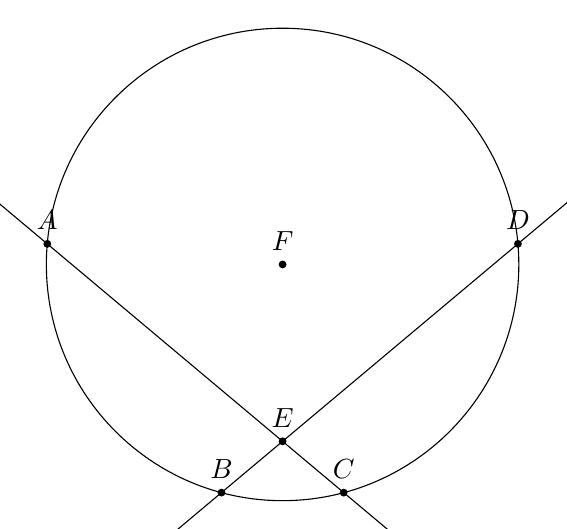
\begin{tikzpicture}[
  dot/.style={circle,inner sep=1pt,fill,label={#1},name=#1},
  dot2/.style={circle,inner sep=1pt,fill},
  extended line/.style={shorten >=-#1,shorten <=-#1},
  extended line/.default=1cm
  ]
\def\radius{3}
\def\ptRadius{0.05} 
\def\at{90+85}
\def\bt{270-15} 
\def\ct{270+15}  
\def\dt{90-85} 
\node[dot=$A$] (A) at ({\radius*cos(\at)},{\radius*sin(\at)}){};   % point on circle
\node[dot=$B$] (B) at ({\radius*cos(\bt)},{\radius*sin(\bt)}){};   % point on circle
\node[dot=$C$] (C) at ({\radius*cos(\ct)},{\radius*sin(\ct)}){};   % point on circle
\node[dot=$D$] (D) at ({\radius*cos(\dt)},{\radius*sin(\dt)}){};   % point on circle
\node[dot=$F$] (F) at (0,0){};                                     % center
\node[dot=$E$] (E) at (intersection of A--C and B--D){};           % intersection E of AB and CD
\draw (F) circle (\radius);
\draw[extended line] (A) -- (C);
\draw[extended line] (B) -- (D);
\end{tikzpicture}
\end{center}

\noindent
Hvis du i sirkelen $ABCD$ lar linjene $AC$ og $BD$ skjære hverandre i et punkt $E$ påstår Euklid at rektangelet med sidelengder $AE$ og $EC$ er lik rektangelet med sidelengder $DE$ og $EB$. Argumentet er som følger: \vspace{1em}

\noindent
Hvis $AC$ og $BD$ går gjennom sentrum, slik at $E$ er sentrum i sirkelen $ABCD$, er det klart at $AE$, $EC$, $DE$ og $EB$ er like og at rektanglene $AE$ ved $EC$ og $DE$ ved $EB$ derfor også er like. Anta nå at $AC$ og $DB$ ikke går gjennom sentrum og la $F$ være sentrum i sirkelen $ABCD$ [III.1]. Trekk nå linjene $FG$ og $FH$ fra $F$ vinkelrett ned på henholdsvis $AC$ og $DB$ [I.12]. Trekk også $FB$, $FC$ og $FE$.

Siden $GF$ går gjennom sentrum i $ABCD$ og skjærer linjen $AC$, som ikke går gjennom sentrum, deler $GF$ linjen $AC$ i to like store deler [III.3]. Altså må $AG$ være lik $GC$. Siden linjen $AC$ har blitt delt i to like store deler av $G$ og i deler av ulik størrelse av $E$ må rektanglet $AE$ ved $EC$ sammen med sammen med kvadratet på $EG$ være lik kvadratet på $GC$ [II.5].

Legg til kvadratet på $GF$ og se at rektanglet $AE$ ved $EC$ sammen med kvadratene på $GE$ og $GF$ er lik summen av kvadratene $CG$ og $GF$. Siden kvadratet på $FE$ er lik summen av kvadratene på $EG$ og $GF$ [I.47], og kvadratet på $FC$ er lik summen av kvadratene $CG$ og $GF$, må rektangelet $AE$ ved $EC$ sammen med kvadratet på $FE$ være lik kvadratet på $FC$.

Siden $FC$ er lik $FB$ må altså rektangelet $AE$ ved $EC$ sammen med kvadratet på $EF$ være lik kvadratet på $FB$. Av samme grunn må også rektangelet $DE$ ved $EB$ sammen med kvadratet på $FE$ være lik kvadratet på $FB$. 

Vi har altså at både rektangelet $AE$ ved $EC$ sammen med kvadratet på $FE$ og rektangelet $DE$ ved $EB$ sammen med kvadratet på $FE$ er lik summen av kvadratene på $FE$ og $FB$. Ved å trekke fra kvadratet $FE$ fra begge sitter vi da igjen med at rektangelet $AE$ ved $EC$ må være lik rektangelet $DE$ ved $EB$.




\begin{center}
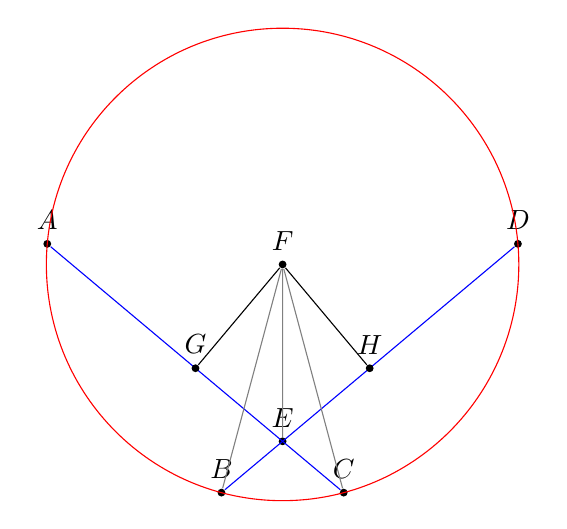
\begin{tikzpicture}[
  dot/.style={circle,inner sep=1pt,fill,label={#1},name=#1},
  dot2/.style={circle,inner sep=1pt,fill},
  extended line/.style={shorten >=-#1,shorten <=-#1},
  extended line/.default=1cm
  ]
\def\radius{3}
\def\ptRadius{0.05} 
\def\at{90+85}
\def\bt{270-15} 
\def\ct{270+15}  
\def\dt{90-85} 
\node[dot=$A$] (A) at ({\radius*cos(\at)},{\radius*sin(\at)}){};   % point on circle
\node[dot=$B$] (B) at ({\radius*cos(\bt)},{\radius*sin(\bt)}){};   % point on circle
\node[dot=$C$] (C) at ({\radius*cos(\ct)},{\radius*sin(\ct)}){};   % point on circle
\node[dot=$D$] (D) at ({\radius*cos(\dt)},{\radius*sin(\dt)}){};   % point on circle
\node[dot=$F$] (F) at (0,0){};                                     % center
\node[dot=$E$] (E) at (intersection of A--C and B--D){};           % intersection E of AB and CD
\draw[red] (F) circle (\radius);
\draw[blue] (A) -- (C);
\draw[blue] (B) -- (D);
\node[dot=$G$] (G) at ($(A)!(F)!(C)$){};
\draw (F) -- (G);
\node[dot=$H$] (H) at ($(B)!(F)!(D)$){};
\draw (F) -- (H);
\draw[gray] (F) -- (B);
\draw[gray] (F) -- (C);
\draw[gray] (F) -- (E);
\end{tikzpicture}
\end{center}


\subsection{I en mer moderne språkdrakt}
Euklids argumentasjon er basert på en tolkning av produkter som faktiske rektangler og linjelengder som par av punkter. La oss forsøke å gjenta argumentene i en mer moderne språkdrakt. \newline

\noindent
La de fire punktene $A,B,C$ og $D$ ligge på en sirkel med sentrum $F$ slik at linjen $AC$ skjærer linjen $BD$ i et punkt $E$. Trekk $FG$ og $FH$ slik at $FG \bot AC$ og $FH \bot BD$. Siden $A,B,C$ og $D$ er punkter på sirkelen må $AG=GC$ og $DH=HB$. Det er et algebraisk faktum at
\EQU{
AE \cdot EC + \left(\frac{AE+EC}{2}-EC\right)^2= \left(\frac{AE+EC}{2}\right)^2
}
og siden $AE+EC=2GC$ og $GC-EC=GE$ kan vi skrive dette som
\EQU{
AE \cdot EC + GE^2= GC^2.
}
Helt tilsvarende har vi også at
\EQU{
BE \cdot ED + HE^2 = HB^2.
}
Trikset er nå å benytte pythagoras. Siden $AC \bot GF$ og $DB \bot HF$ må $HF^2 + HE^2 = EF^2$ og $GF^2+GE^2=EF^2$ og derfor
\EQU{
AE \cdot EC + EF^2= GC^2 + GF^2 \mbox{ og } BE \cdot ED + EF^2 = HB^2 + HF^2.
}
Men $GC \in AB$ og $HB \in BD$ så pythagoras gjelder også her. Da må
\EQU{
AE \cdot EC + EF^2= FC^2 \mbox{ og } BE \cdot ED + EF^2 = FB^2
}
og siden $B$ og $C$ ligger på sirkelen må $EF=FB$. Da må
\EQU{
AE \cdot EC = BE \cdot ED,
}
som er det vi ønsket å vise.


\subsection{Et mer moderne bevis}
Vi har nå sett hvordan Euklids originale argument kan oversiktliggjøres av å introdusere det algebramaskineriet som har kommet etter Euklids tid. Euklids argument bærer imidlertid både preg av \textit{elementers} oppbygning og datidens manglende formalisme. Av den grunn presenterer jeg også et alternativ, og kanskje hakket mer moderne, bevis. \newline

\begin{multicols}{2}

\begin{center}
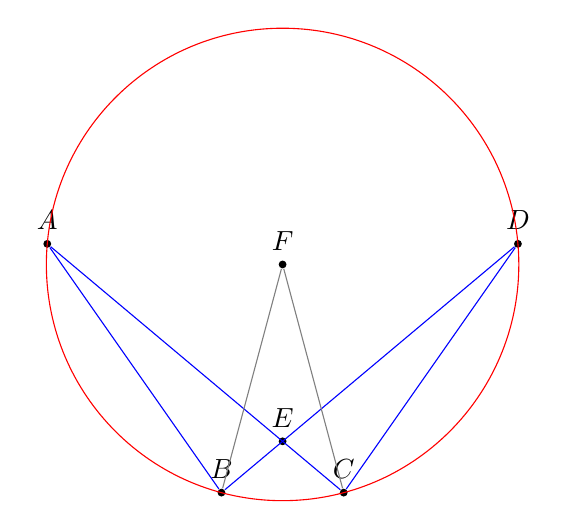
\begin{tikzpicture}[
  dot/.style={circle,inner sep=1pt,fill,label={#1},name=#1},
  dot2/.style={circle,inner sep=1pt,fill},
  extended line/.style={shorten >=-#1,shorten <=-#1},
  extended line/.default=1cm
  ]
\def\radius{3}
\def\ptRadius{0.05} 
\def\at{90+85}
\def\bt{270-15} 
\def\ct{270+15}  
\def\dt{90-85} 
\node[dot=$A$] (A) at ({\radius*cos(\at)},{\radius*sin(\at)}){};   % point on circle
\node[dot=$B$] (B) at ({\radius*cos(\bt)},{\radius*sin(\bt)}){};   % point on circle
\node[dot=$C$] (C) at ({\radius*cos(\ct)},{\radius*sin(\ct)}){};   % point on circle
\node[dot=$D$] (D) at ({\radius*cos(\dt)},{\radius*sin(\dt)}){};   % point on circle
\node[dot=$F$] (F) at (0,0){};                                     % center
\node[dot=$E$] (E) at (intersection of A--C and B--D){};           % intersection E of AB and CD
\draw[red] (F) circle (\radius);
\draw[blue] (A) -- (C);
\draw[blue] (A) -- (B);
\draw[blue] (D) -- (C);
\draw[blue] (D) -- (B);
\draw[gray] (F) -- (B);
\draw[gray] (F) -- (C);
\end{tikzpicture}
\end{center}
\vspace{1cm}

\noindent
La de fire punktene $A,B,C$ og $D$ ligge på en sirkel med sentrum $F$ slik at linjen $AC$ skjærer linjen $BD$ i et punkt $E$. Planen er å vise at trekantene $\Delta AEB$ og $\Delta DEC$ er formlike. Siden $\angle AEB = \angle DEC$ holder det på vise likhet blant en av de andre vinklene. Da kan det være fint å observere at $\angle BAC = \frac{1}{2}\angle BFC$ siden en periferivinkel alltid er halvparten så stor som gradtallet til sirkelbuen utspent av vinkelens ben. Dette er jo også sant for den andre vinkelen. Da må $\angle BDC = \frac{1}{2} \angle BDC = \angle BAC$. Altså er alle vinklene like i de to trekantene, og derfor er $\Delta AEB$ formlik $\Delta DEC$. Per definisjon av formlikhet er da $AE\cdot EC = DE \cdot EB$.

\end{multicols}

\subsection{Punkt utenfor sirkelen}

\begin{multicols}{2}
\noindent
Proposisjon 35 i bind tre introduserer en pussig egenskap til punkter i en sirkels indre; enhver korde gjennom punktet vil av punktet deles slik at produktet av segmentene er uavhengig av korden. Det er da naturlig å undersøke hvorvidt dette også gjelder når punktet ligger utenfor sirkelen. Problemet er da at proposisjon II.5 faller sammen -- når $D$ ikke deler $AB$ blir kvadratet på $CD$ større enn kvadratet på $CB$. Dette ville imidlertid ikke vært noe problem dersom rektangelet $AD$ ved $DB$ var negativt, hva enn det betyr. Hvis vi fjerner oss fra tolkningen av produktet $AD\cdot DB$ som et rektangel, er det ikke noe problem dersom dette skulle vise seg å være negativt. Vi kan simpelthen introdusere et fortegnsmål og konstatere at for et punkt $P$ er relasjonen
\EQU{
AP\cdot PB = CP\cdot PD
}
alltid oppfylt for punkter $A,B,C$ og $D$ som ligger på en sirkel slik at punktet $P$ er skjæringspunktet for de to linjene $AB$ og $CD$.

\vspace{2cm}

\begin{center}
\begin{tikzpicture}[
  dot/.style={circle,inner sep=1pt,fill,label={#1},name=#1},
  dot2/.style={circle,inner sep=1pt,fill},
  extended line/.style={shorten >=-#1,shorten <=-#1},
  extended line/.default=1cm
  ]
\def\radius{3}
\def\ptRadius{0.05} 
\def\at{90+85}
\def\ct{270-15} 
\def\bt{270+15}  
\def\dt{90-85} 
\node[dot=$A$] (A) at ({\radius*cos(\at)},{\radius*sin(\at)}){};   % point on circle
\node[dot=$B$] (B) at ({\radius*cos(\bt)},{\radius*sin(\bt)}){};   % point on circle
\node[dot=$C$] (C) at ({\radius*cos(\ct)},{\radius*sin(\ct)}){};   % point on circle
\node[dot=$D$] (D) at ({\radius*cos(\dt)},{\radius*sin(\dt)}){};   % point on circle
\node[dot=$S$] (S) at (0,0){};                                     % center
\node[dot=$P$] (P) at (intersection of A--C and B--D){};           % intersection E of AB and CD
\draw[red] (F) circle (\radius);
\node[dot=$G$] (G) at ($(A)!(F)!(C)$){};
\draw (F) -- (G);
\node[dot=$H$] (H) at ($(B)!(F)!(D)$){};
\draw (F) -- (H);
\draw[blue] (A) -- (P);
\draw[blue] (A) -- (B);
\draw[blue] (D) -- (C);
\draw[blue] (D) -- (P);
\end{tikzpicture}
\end{center}

\end{multicols}

\noindent
Ettersom det iblant kan være ugreit å holde styring på fortegnsmålet kan det være lurt heller å studere den negative påstanden. Siden $CP=-PC$ og $AP=-PA$ følger det at
\EQU{
PA \cdot PB = PC \cdot PD. 
}
Denne størrelsen kalles gjerne for \textit{potensen til punktet $P$ i forhold til sirkelen}. Siden verdien er uavhening av punktene kan vi velge en linje som skjærer sentrum i sirkelen. Dersom avstanden fra punktet $P$ til sentrum i sirkelen er $a$ og radien i sirkelen er $r$, er punktets potens $p(P)$ gitt av uttrykket
\EQU{
p(P)=(a+r)(a-r)=a^2-r^2.
}
Det er da tydelig at potensen til punktet $P$ i forhold til sirkelen er positivt når $P$ ligger utenfor sirkelen, og negativt når $P$ ligger i sirkelens indre. For punkter utenfor sirkelen ser det ut til at punktets potens er kvadratet på kateten til en eller annen rettvinklet trekant med hypotenus lik $a$ og sidelengde $r$. Med andre ord vil en sirkel rundt det ytre punktet $P$ med radius $\sqrt{p(P)}$ alltid skjære den originale sirkelen i rette vinkler. Vi sier da at de to sirklene er orthogonale.

\begin{center}
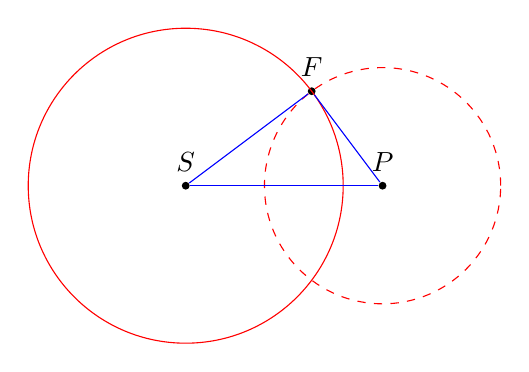
\begin{tikzpicture}[
  dot/.style={circle,inner sep=1pt,fill,label={#1},name=#1},
  dot2/.style={circle,inner sep=1pt,fill},
  extended line/.style={shorten >=-#1,shorten <=-#1},
  extended line/.default=1cm
  ]
\def\r{2}
\def\a{2.5}
\def\R{sqrt(\a*\a - \r*\r)}
\def\v{asin(\R/\a)}
\node[dot=$S$] (S) at (0,0){};                 
\node[dot=$P$] (P) at (\a,0){}; 
\node[dot=$F$] (F) at ({\r*cos(\v)},{\r*sin(\v)}){};
\draw[red] (S) circle (\r);
\draw[red,dashed] (P) circle (\R);
\draw[blue] (S) -- (P);
\draw[blue] (S) -- (F);
\draw[blue] (F) -- (P);
\end{tikzpicture}
\end{center}


\subsection{Darbouxproduktet}
I figuren over så vi hvordan vi kan tolke potensen til et punkt $P$ utenfor sirkelen som kvadratet av radien til sirkelen rundt $P$ som skjærer den originale sirkelen i rette vinkler. Dersom vi i figuren over introduserer navnene $a=SP$, $r_1 = SF$ og $r_2 = PF$ har vi altså at $a^2-r_1^2-r_2^2=0$. Den størrelsen som her er null, kalles for \textit{Darbouxproduktet} mellom de to sirklene. For to sirkler $S_1$ og $S_2$, med sentum i henholdsvis $A_1$ og $A_2$ og med radius $r_1$ og $r_2$, er Darbouxproduktet mellom de to sirklene gitt av
\EQU{
D(S_1,S_2) = (A_1 A_2)^2-r_1^2-r_2^2.
}

\begin{multicols}{3}
\begin{center}
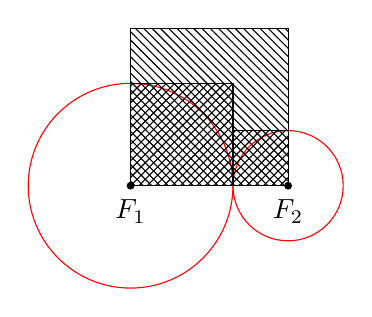
\begin{tikzpicture}[
  dot/.style={circle,inner sep=1pt,fill,label=below:{#1},name=#1},
  dot2/.style={circle,inner sep=1pt,fill},
  extended line/.style={shorten >=-#1,shorten <=-#1},
  extended line/.default=1cm
  ]
\def\r{1.3}
\def\R{0.7}
\def\a{2}
\node[dot=$F_1$] (F1) at (0,0){};
\node[dot=$F_2$] (F2) at (\a,0){};   
\draw[red] (F1) circle (\r);
\draw[red] (F2) circle (\R);
\draw[blue] (F1) -- (F2);
\draw [pattern=north west lines] (F1) rectangle (\a,\a);
\draw [pattern=north east lines]   (F1) rectangle (\r,\r);
\draw [pattern=north east lines]   (F2) rectangle (\a-\R,\R);
\end{tikzpicture}
\end{center}

\noindent
Legg merke til at dersom radien i $S_2$ blir uendelig liten, sitter vi igjen med uttrykket $D(S_1,S_2) = (A_1 A_2)^2-r_1^2$, som ikke er annet en potensen til punktet $A_2$ med hensyn på sirkelen $S_1$.

\begin{center}
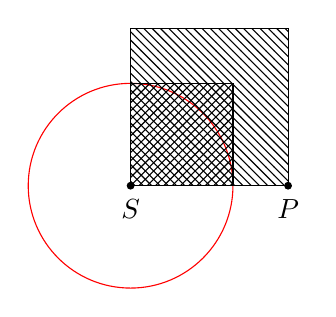
\begin{tikzpicture}[
  dot/.style={circle,inner sep=1pt,fill,label=below:{#1},name=#1},
  dot2/.style={circle,inner sep=1pt,fill},
  extended line/.style={shorten >=-#1,shorten <=-#1},
  extended line/.default=1cm
  ]
\def\r{1.3}
\def\R{0}
\def\a{2}
\node[dot=$S$] (F1) at (0,0){};
\node[dot=$P$] (F2) at (\a,0){};   
\draw[red] (F1) circle (\r);
\draw[red] (F2) circle (\R);
\draw[blue] (F1) -- (F2);
\draw [pattern=north west lines] (F1) rectangle (\a,\a);
\draw [pattern=north east lines]   (F1) rectangle (\r,\r);
\draw [pattern=north east lines]   (F2) rectangle (\a-\R,\R);
\end{tikzpicture}
\end{center}
\end{multicols}

\noindent
Vi kan, ved å stirre lenge på uttrykket, dra kjensel på noe som vi i løpet av folkeskolen lærte å kalle \textit{cosinussetningen}. Dersom de to sirklene skjærer hverandre med en vinkel $\theta$ kan vi skrive
\EQU{
D(S_1,S_2) = -2r_1 r_2 \cos \theta,
}
som tydeliggjør hvorfor produktet er null når sirklene er orthogonale. 



\subsection{Punkter med lik potens}
La oss skape to sirkler, én med sentrum i $S_1$ og radius $r_1$ og én med sentrum i $S_2$ og radius $r_2$, som skjærer hverandre i to punkter $K_1$ og $K_2$. Vi kan da introdusere et punkt $P$ og la $a_1=S_1 P$ og $a_2 = S_2 P$. Siden $a_1^2-a_2^2$ nødvendigvis må være en lineær funksjon av $P$ følger det at differansen mellom potensen $p_1(P)$ og potensen $p_2(P)$ til $P$ med hensyn på henholdsvis sirkel $1$ og sirkel $2$, er en lineær funksjon av $P$. Ved å bruke koordinattransformasjonen $\vec{S_1}=\vec{0}$, $\vec{S_2}=a_x\hat{i}+a_y\hat{j}$ og $\vec{P}=x\hat{i}+y\hat{j}$ fremstår dette også tydelig ved
\EQU{
p_1(\vec{P})-p_2(\vec{P})=x^2+y^2-r_1^2-\left[ (x-a_x)^2+(y-a_y)^2-r_2^2 \right] = 2xa_x+2ya_y+r_2^2-r_1^2-a_x^2-a_y^2.
}
Dersom vi skulle ønske å finne ut hvilke punkter $P$ som har lik potens i forhold til de to sirklene vet vi altså at svaret er en eller annen rett linje. Ettersom punkter langs randen av en sirkel alltid har potens lik null må punktene $K_1$ og $K_2$, som ligger på begge sirklenes rand, ha lik potens med hensyn på begge sirklene. Da følger det at linjen som inneholder alle punktene $P$ med samme potens i forhold til begge sirklene er linjen $K_1K_2$.

\begin{center}
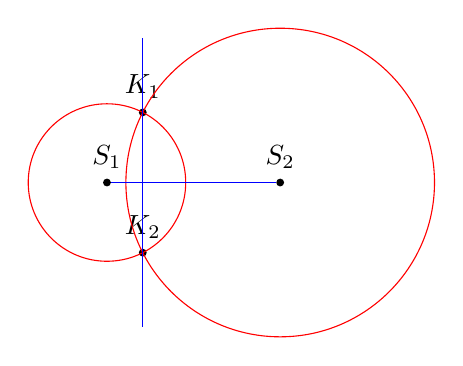
\begin{tikzpicture}[
  dot/.style={circle,inner sep=1pt,fill,label={#1},name=#1},
  dot2/.style={circle,inner sep=1pt,fill},
  extended line/.style={shorten >=-#1,shorten <=-#1},
  extended line/.default=1cm
  ]
\def\r{1}
\def\a{2.2}
\def\R{sqrt(\a*\a - \r*\r)}
\def\v{+asin(\R/\a)}
\def\w{-asin(\R/\a)}
\node[dot=$S_1$] (S1) at (0,0){};                 
\node[dot=$S_2$] (S2) at (\a,0){}; 
\node[dot=$K_1$] (K1) at ({\r*cos(\v)},{\r*sin(\v)}){};
\node[dot=$K_2$] (K2) at ({\r*cos(\w)},{\r*sin(\w)}){};
\draw[red] (S1) circle (\r);
\draw[red] (S2) circle (\R);
\draw[blue] (S1) -- (S2);
\draw[blue,extended line] (K1) -- (K2);
\end{tikzpicture}
\end{center}

\noindent
Denne linjen kalles \textit{potenslinjen} for de to sirklene. Dersom $F$ er et punkt på denne linjen vil sirkelen med radius $\sqrt{p(F)}$ alltid være orthogonal på begge sirklene. Vi kunne her begynt å studere skjæringspunktet mellom potenslinjer, eller mer interessant, skjæringspunktet mellom potenslinjen og linjen $SP$. Vi kunne studert hvordan ulike mengder oppfører seg under avbildningen som bytter ytre punkter for en sirkel med skjæringspunktet mellom potenslinjen og linjen mellom punktet og sentrum i sirkelen. Her ville vi oppdaget det området i matematikk som går under navnet \textit{invers geometri}, men dette er en tekst som er viet til proposisjon III.35 i Euklids elementer. Av den grunn avslutter vi med en illustrasjon av 2000 sirkler jevnt fordelt langs en potenslinje sammen med de to orthogonale sirklene som er opphav til potenslinjen.


\begin{center}
\includegraphics[width=0.95\textwidth]{potenslinje.png}
\end{center}








\begin{thebibliography}{99} % Bibliography - this is intentionally simple in this template
 
 \bibitem{DEJ:IIIprop35}
 David E. Joyce (1996)
 \newblock Euclid's Elements Book III, Proposition 35. [lest 3. Nov 2015]
 \newblock \newline
   \small{\url{http://aleph0.clarku.edu/~djoyce/java/elements/bookIII/propIII35.html}}.

\bibitem{WIKI:Elements}
 Wikipedia
 \newblock Euclid's Elements. [lest 3. Nov 2015]
 \newblock \newline
   \small{\url{https://en.wikipedia.org/wiki/Euclid's_Elements}}.


\bibitem{WIKI:PotensTilPunkt}
 Wikipedia
 \newblock Power of a point. [lest 3. Nov 2015]
 \newblock \newline
   \small{\url{https://en.wikipedia.org/wiki/Power_of_a_point}}.

 \bibitem{WIKI:Oxyrhynchus}
  Wikipedia
  \newblock Papyrus Oxyrhynchus 29. [lest 4. Nov 2015]
  \newblock \newline
    \small{\url{https://en.wikipedia.org/wiki/Papyrus_Oxyrhynchus_29}}.
 
 
\end{thebibliography}





\end{document}
